\subsection{Installing \emph{mono}}
\label{sec:mono}
This is a step-by-step guide to install \emph{mono} the cluster. In total it takes about 1 hour to finish the installation!
\begin{enumerate}
\item Go to the developers homepage \url{http://download.mono-project.com/sources/mono/} and copy the link of your desired %mono version (\verb|$mono-link|). As of December 2017 mono-5.9.0.415 is tested and working.
\item Open a git bash and login on one of the four login nodes of the cluster, e.g 1
\begin{verbatim}
ssh $TuID@$host
\end{verbatim}
\item Create a new directory \verb|mono| in \verb|$home| and open it
\begin{verbatim}
mkdir mono
cd mono
\end{verbatim}
\item Download the \emph{mono} archive into the directory
\begin{verbatim}
wget $mono-link
\end{verbatim}
\item Open \emph{mono} archive
\begin{verbatim}
tar -xjf mono-x.x.x.tar.bz2
\end{verbatim}
\item open the created folder
\begin{verbatim}
cd mono-x.x.x
\end{verbatim}
\item before compilation, mono has to be configured, which requires \emph{cmake}. Prefix gives the directory for the binaries (these are two commands)
\begin{verbatim}
module load cmake
./configure --prefix=/home/$TuID/mono/mono-x.x.x_bin
\end{verbatim} 
\item After a successful configuration the compilation can be started
\begin{verbatim}
make
\end{verbatim}
It can happen that the compiler ask for additional prompts. Just type \verb|.| and return.
The whole compilation takes about 50-60 minutes!
\item to finish the installation prompt
\begin{verbatim}
make install
\end{verbatim} 
\item Finally \emph{mono} has to be added to the \verb|PATH| and \verb|LD_LIBRARY_PATH| variable. This can be done in the .bashrc file: Go back to your \verb|$home| directory and open the .bashrc with an editor, e.g. vi
\begin{verbatim}
cd ~
vi .bashrc
\end{verbatim}
add to following lines for the \verb|PATH| variable (press \emph{i} to insert text)
\begin{verbatim}
PATH=/home/$TuID/mono/mono-x.x.x_bin/bin:$PATH
export PATH
\end{verbatim}
and for the \verb|LD_LIBRARY_PATH| variable
\begin{verbatim}
LD_LIBRARY_PATH=/home/$TuID/mono/mono-x.x.x_bin/lib:$LD_LIBRARY_PATH
export LD_LIBRARY_PATH
\end{verbatim}
Press \emph{Esc} and type \emph{:wq} to save your latest changes and quit the application. Save the changes and reload .bashrc by prompting
\begin{verbatim}
source .bashrc
\end{verbatim}
\end{enumerate} 

\subsection{Installing \emph{HYPRE}}
\label{sec:hypre}
NOTE: hypre is not used anymore by \Bosss. The former used binary can be found in \verb|$BoSSSNetDrive\binaries\hhlr\Hypre|.

Installing \emph{HYPRE} works similar to the installation routine of \emph{mono} (see section \ref{sec:mono}). Hence only the bash commands are given:
\begin{enumerate}
\item go to the developers homepage \url{http://computation.llnl.gov/casc/hypre/software.html} and copy the link of your desired hypre version (\verb|$hypre-link|). 
\item login on the cluster
\begin{verbatim}
ssh $TuID@$host
\end{verbatim}
\item 
\begin{verbatim}
mkdir hypre
cd hypre
\end{verbatim}
\item 
\begin{verbatim}
wget $hypre-link
\end{verbatim}
\item Note the different tar command
\begin{verbatim}
tar -xzf hypre-x.x.x.tar.gz
\end{verbatim}
\item 
\begin{verbatim}
cd hypre-x.x.x/src
\end{verbatim}
\item Note the additional command --enable-shared 
\begin{verbatim}
./configure --prefix=/home/$TuID/hypre/hypre-x.x.x_bin --enable-shared
\end{verbatim} 
\item 
\begin{verbatim}
make
\end{verbatim}
\item
\begin{verbatim}
make install
\end{verbatim} 
\item only the \emph{HYPRE} library is used thus only the \verb|LD_LIBRARY_PATH| variable has to be adjusted in .bashrc
\begin{verbatim}
cd ~
vi .bashrc
\end{verbatim}
and add
\begin{verbatim}
LD_LIBRARY_PATH=/home/$TuID/hypre/hypre-x.x.x_bin/lib:$LD_LIBRARY_PATH
export LD_LIBRARY_PATH
\end{verbatim}
save the changes and reload .bashrc by prompting
\begin{verbatim}
source .bashrc
\end{verbatim}
\end{enumerate} 

\subsection{Installing \emph{ParMETIS}}
\label{sec:parmetis}
BoSSS does not work with the latest version of \emph{ParMETIS}. Therefore an older version is needed. You can find the binary in the BoSSS repository.
\begin{enumerate}
\item copy the \emph{ParMETIS} binary folder on the cluster
\begin{verbatim}
scp -r $BoSSSDir/public/src/ilPSP/layer_0/3rd_party/ParMETIS $TuID@$host:~/ParMETIS/
\end{verbatim}
\item login on the cluster
\begin{verbatim}
ssh $TuID@$host
\end{verbatim}
\item build \emph{ParMETIS} using the bash-script \emph{buildParMETIS.sh}
\begin{verbatim}
cd ~/ParMETIS
dos2unix buildParMETIS.sh
bash buildParMETIS.sh
\end{verbatim}
\item  add the \emph{ParMETIS} library to the \verb|LD_LIBRARY_PATH| variable in .bashrc
\begin{verbatim}
vi .bashrc
\end{verbatim}
and add
\begin{verbatim}
LD_LIBRARY_PATH=/home/$TuID/ParMETIS/:$LD_LIBRARY_PATH
export LD_LIBRARY_PATH
\end{verbatim}
\end{enumerate}
Note: \verb|export LD_LIBRARY_PATH| needs only to be called once after the last change of the \verb|LD_LIBRARY_PATH|.\\\\
\textit{Remark: If it does not compile it is easier to use the compiled binaries instead. You can find them in} \verb|$BoSSSNetDrive\binaries\hhlr\ParMETIS|
Note: You find \emph{ParMETIS} only in the GridOfTomorrow branch!

 this is obsolete, we are yousing Intel's Pardiso(MKL) now ...
\subsection{Installing \emph{PARDISO V5}}
\begin{enumerate}
\item download the newest \emph{PARDISO} Version from the Website \emph{http://www.pardiso-project.org} or from \verb|\\scratch\kummer\pardiso.zip| and copy the \verb|.so|-file to \verb|\home\$TUID/PARDISO|
\item  add the \emph{PARDISO} library to the \verb|LD_LIBRARY_PATH| variable in .bashrc
\begin{verbatim}
vi .bashrc
\end{verbatim}
and add
\begin{verbatim}
LD_LIBRARY_PATH=/home/$TuID/PARDISO:$LD_LIBRARY_PATH
export LD_LIBRARY_PATH
\end{verbatim}
\item get a licence from the pardiso website
\item open PardisoSolver.cs of your version of BoSSS
\item change Version m\_Version = Version.MKL to Version m\_Version = Version.v5 and add your licence key in between the quotation marks as seen below
%\item add the following to your xml-file
%\begin{verbatim}
%	  <sparsesolver name="PARDISO-V5">
%	    <type>direct</type>
%	    <library>pardiso</library>
%	    <specific>
%	      <Version>v5</Version>
%	      <!-- username '$TUID', (Lichtenberg) no NODE-lock : -->
%	      <LicenseCode>PUT LICENCE CODE HERE</LicenseCode>
%	    </specific>
%	  </sparsesolver>
%\end{verbatim}
\end{enumerate}
\begin{figure}[htbp] % htb: preferred position of picture: here, top, bottom of page
	\begin{centering}
		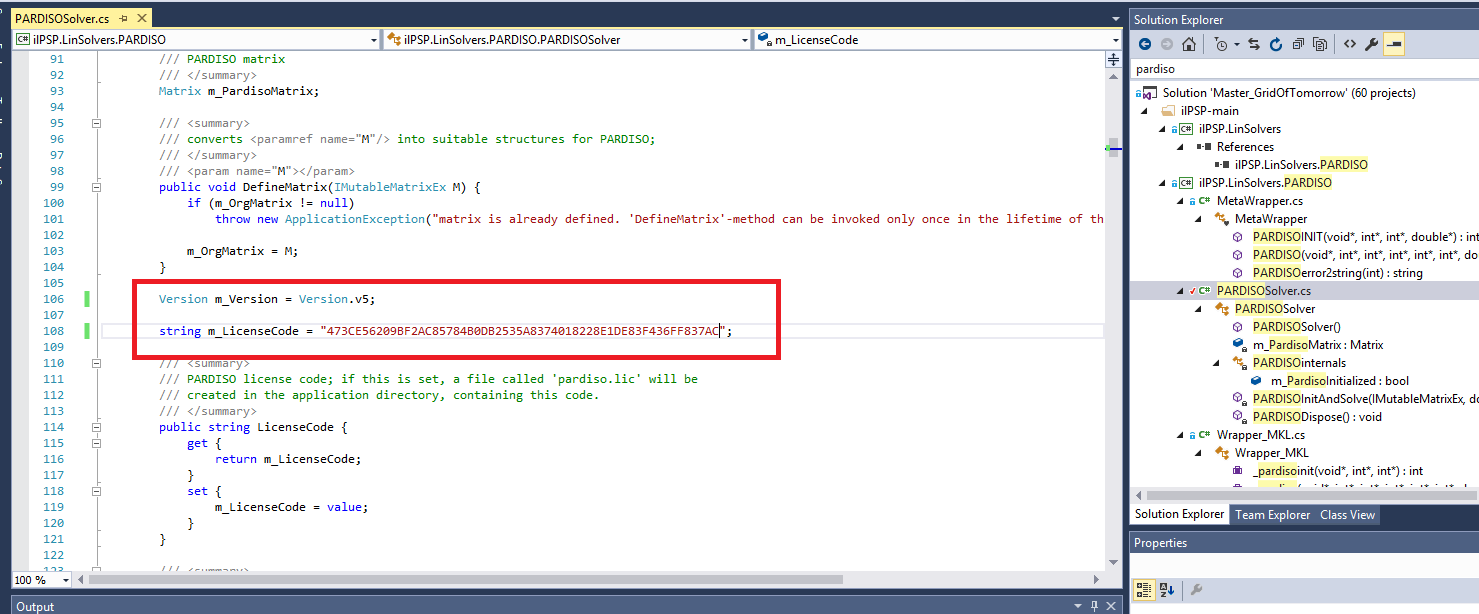
\includegraphics[width=0.9\textwidth]{Figures/pardiso_licence.png}\\
	\end{centering}
	\caption{Add your key to the Pardiso Solver}\label{fig:pardiso_licence}
\end{figure} %

\subsection{Installing \emph{MUMPS V5.0.2}}
\label{sec:mumps}
In the following the compilation of MUMPS on the Lichtenberg cluster will be explained.
\begin{enumerate}
	\item Download MUMPS\_5.0.2 from the MUMPS website and unzip it.
	\item Copy the \textbf{Makefile.inc} into the main MUMPS folder and the \textbf{build\_shared} script to the \textit{/lib} directory. You can find both files in the underlying folder \textit{Lichtenberg} in the same directory as this document.
	\item Load modules \textbf{intel/2016u4} (2017 does not work) and one \textbf{openmpi/intel/2.0.1}.
	\item Execute the makefile by typing 'make'.
	\item If all went well there should be three libraries, naming libdmumps.a, libmumps\_common.a and libpord.a in your \textit{/lib} folder.
	\item Open the \textbf{build\_shared} and adjust the path to a folder in your home directory
	\item Execute the \textbf{build\_shared} by typing './build\_shared'. If you do not get permission to execute it, copy each line and run them separately.
	\item Modify your \textbf{.bashrc} and add the path to your libdmumps.so.	
\end{enumerate}
Now it should be possible to run the MUMPS solver on the Lichtenberg cluster in the same way you do on windows. 

The performance of MUMPS can possibly be increased by linking against Metis and Parmetis. At this stage there was a conflict between BoSSS, using Parmetis 3 and MUMPS, using Parmetis 4. As a reason the software Pord, which is distributed with MUMPS is being used for partitioning.